\documentclass[11 pt, a4paper]{article}  % list options between brackets
\usepackage[nottoc,notlof,notlot,numbib]{tocbibind}
\usepackage[margin=1.1 in]{geometry}
\usepackage{fancyhdr}
\usepackage{manfnt}
\usepackage{pgf}
\usepackage{amsmath,amssymb,natbib,graphicx}
\usepackage{amsfonts}
\DeclareMathAlphabet{\mathpzc}{OT1}{pzc}{m}{it}
\usepackage{bbm}
\usepackage{hyperref}
\usepackage{float}
\usepackage{mathrsfs} %mathscr{A}
\usepackage{subfigure}
\usepackage{chngpage}

\usepackage{times}
\usepackage{latexsym}
\usepackage{caption}

\usepackage{algorithm}
\usepackage[noend]{algpseudocode}

\newtheorem{axiom}{Axiom}[section]
\newtheorem{result}{Result}[section]
\newtheorem{example}{example}[section]
\newtheorem{definition}{Definition}[section]
\newtheorem{principle}{Principle}[section]
\newtheorem{theorem}{Theorem}[section]% list packages between braces

% type user-defined commands here
%\newcommand{\vmu}{{\bf \mu}}
%\newcommand{\vtheta1}{{\bf \theta^{(1)}}}
%\newcommand{\vtheta2}{{\bf \theta^{(2)}}}
%\newcommand{\vpi}{{\bf \pi}}}

\newcommand{\gm}{\gamma}

\begin{document}

\title{Summary of Short-term Research Objectives}   % type title between braces
\author{Detian Deng}         % type author(s) between braces
\date{\today}    % type date between braces
\maketitle

%\begin{abstract}
%\end{abstract}



\section{Log Linear Model Representation}             % section 1
Let $L$ be a K-dimensional Bernoulli random variable denoting the true state.
Consider the general log linear model:
\begin{align*}
f(l; \Theta) = & \exp \{\Theta_1^T l + \Theta_2^{T} u_2 + \ldots + \Theta_K^T u_K - A^*(\Theta)\}
\end{align*}
where $U_k$ is a ${K \choose k} \times 1$ vector of k-way cross-products, $k = 1,\ldots,K$,  and $\Theta = (\Theta_1,\ldots, \Theta_K)$ contains the the natural parameters, which is a $(2^K-1) \times 1$ vector.\\
\ \\
Model restrictions, let $\tilde{l} = (l,u_2,\dots,u_K)^T$, and $S = \sum_{j=1}^K L_j = s$ has some fixed pmf 
\begin{align}
\pi(s) := & P(S=s)\nonumber \\ 
= & \frac{1}{A(\Theta)} \sum_{\tilde{l}:S=s}\exp \{ \Theta^T \tilde{l}\}  \text{ , } s = 0,1,\ldots, K \\
A(\Theta) = & \sum_{\tilde{l}:l\in \{0,1\}^K}\exp \{ \Theta^T \tilde{l}\}
\end{align}

For the saturated log linear model, $\tilde{L}$ is a square matrix with dimension $J_1 = 2^K-1$. Recall that 
\begin{align}
A(\Theta) = & \frac{1}{\pi(0)} \nonumber \\
\pi(s) = & \frac{1}{A(\Theta)} \sum_{\tilde{l}:S=s}\exp \{ \Theta^T \tilde{l}\}  \text{ , } s = 1,\ldots, K \\
\mu_k = & \frac{1}{A(\Theta)} \sum_{\tilde{l}:l_k=1}\exp \{ \Theta^T \tilde{l}\}  \text{ , } k = 1, \ldots, K
\end{align}
Define intermediate parameter $\phi_j = \exp(\theta^T\tilde{l}_j) >0$, $\Theta = (\theta^{(1)},\theta^{(2)}, \ldots, \theta^{(K)}), j= 1, \ldots, J_1$ and two $K \times J_1$ sub-design matrices $B$, $C$, where $B[k,j] = 1(\sum_{s=1}^K\tilde{L}[j,s]=k)$, $C[k,j] = \tilde{L}[j,k]$. Thus (3) and (4) become
\begin{align}
\vec{\phi} > & 0\\
B \vec{\phi} = & \vec{\pi}/\pi(0)\\ 
C \vec{\phi} = & \vec{\mu}/\pi(0)
\end{align}
Note that B and C are not independent constraints and should be compatible so that $\binom{B}{C}$ has rank $2K-1$.
Explicitly, $\mu$ and $\pi$ must satisfy  
\[ \sum_{k=1}^K \mu_k = \sum_{k=1}^K k\pi_k\]
Based on [1][2], we can sample $\vec{\phi}$ from Uniform distribution subject to the above linear constraints efficiently and robustly. Then $\Theta$ are the solutions to the linear system ($J_1$ equations with $J_1$ unknowns):
\[\tilde{L}\Theta = \log \vec{\phi}\]


\section{Multinomial Representation}
Considering all possible outcomes of the K-dimensional Bernoulli random vector as a $2^K$-dimensional Multinomial random vector, if all the Multinomial cell probabilities are strictly positive, then there is a a one-to-one mapping between the cell probabilities $p$ and the canonical parameters $\Theta$ in the saturated log linear model through the intermediate parameters $\phi$ defined above.
\begin{align*}
p_0 = & \pi_0 = \frac{1}{1+\sum \phi_j}\\
p_j = & \pi_0 \phi_j
\end{align*}

\subsection{Sparsity of Multinomial Model}
If we allow some of the cell probabilities to be exactly 0, then the model violates the log linear model framework, but gains useful model sparsity to our interests and the above relations among $\mu$, $\pi$, $\phi$ and $p$ still hold.\\

In the etiology study, scientists have strong beliefs that there cannot be too many (like more than 3) pathogens that jointly cause the disease. In other words, for some fixed integer $1\leq S_{max} \leq K$, P($S > S_{max}$) = 0. And we can make use of this belief by taking it into the specification of prior and likelihood function.
  

\section{Model without Measurement Error}
The posterior density $P(\mu, \pi | L)$ is proportional to the joint density $P(\mu, \pi, L) = P(L | \mu, \pi)P(\mu,\pi)$. We can sample from the posterior distribution by Metropolis-Hastings Algorithm as long as we define the likelihood and prior properly. 
\subsection{The Prior $P(\mu, \pi)$}
\[P(\mu,\pi) =  P(\pi) P(\mu | \pi)\]
$P(\pi) = P(\pi; \alpha)$, where $(\pi_{Smax+1}, \ldots, \pi_K)=0$ and $(\pi_0,\ldots, \pi_{S_{max}}) \sim$ Dirichlet$(\alpha)$. \\
$P(\mu | \pi)$ is a uniform distribution for $\mu$ in $(0,1-\pi_0)^K$ subject to the linear constrain:
\[ \sum_{k=1}^K \mu_k = \sum_{k=1}^{S_{max}} k\pi_{k}\]
Since we know that the sum of independent standard uniform random variable follows Irwin-Hall distribution, it can be shown that this conditional density has a closed form as follow, where $q = 1-\pi_0$ and $Q=\sum_{k=1}^{S_{max}} k\pi_{k}$
\[ P(\mu | \pi) = q^K \Big \{\frac{1}{2q(K-1)!} \sum_{k=0}^K (-1)^k {K \choose k} (Q/q-k)^{K-1} \text{sign}(Q-kq) \Big \}^{-1} \]
Therefore, $\alpha$ controls the informative part of the prior on $\pi$ and a conditional non-informative prior is set on $\mu$. For example, with $K=5, S_{max}=3, \alpha=(1,4,2,1)$, the prior marginal density of $(\mu, \pi)$ is shown in Fig \ref{prior}

\begin{center}
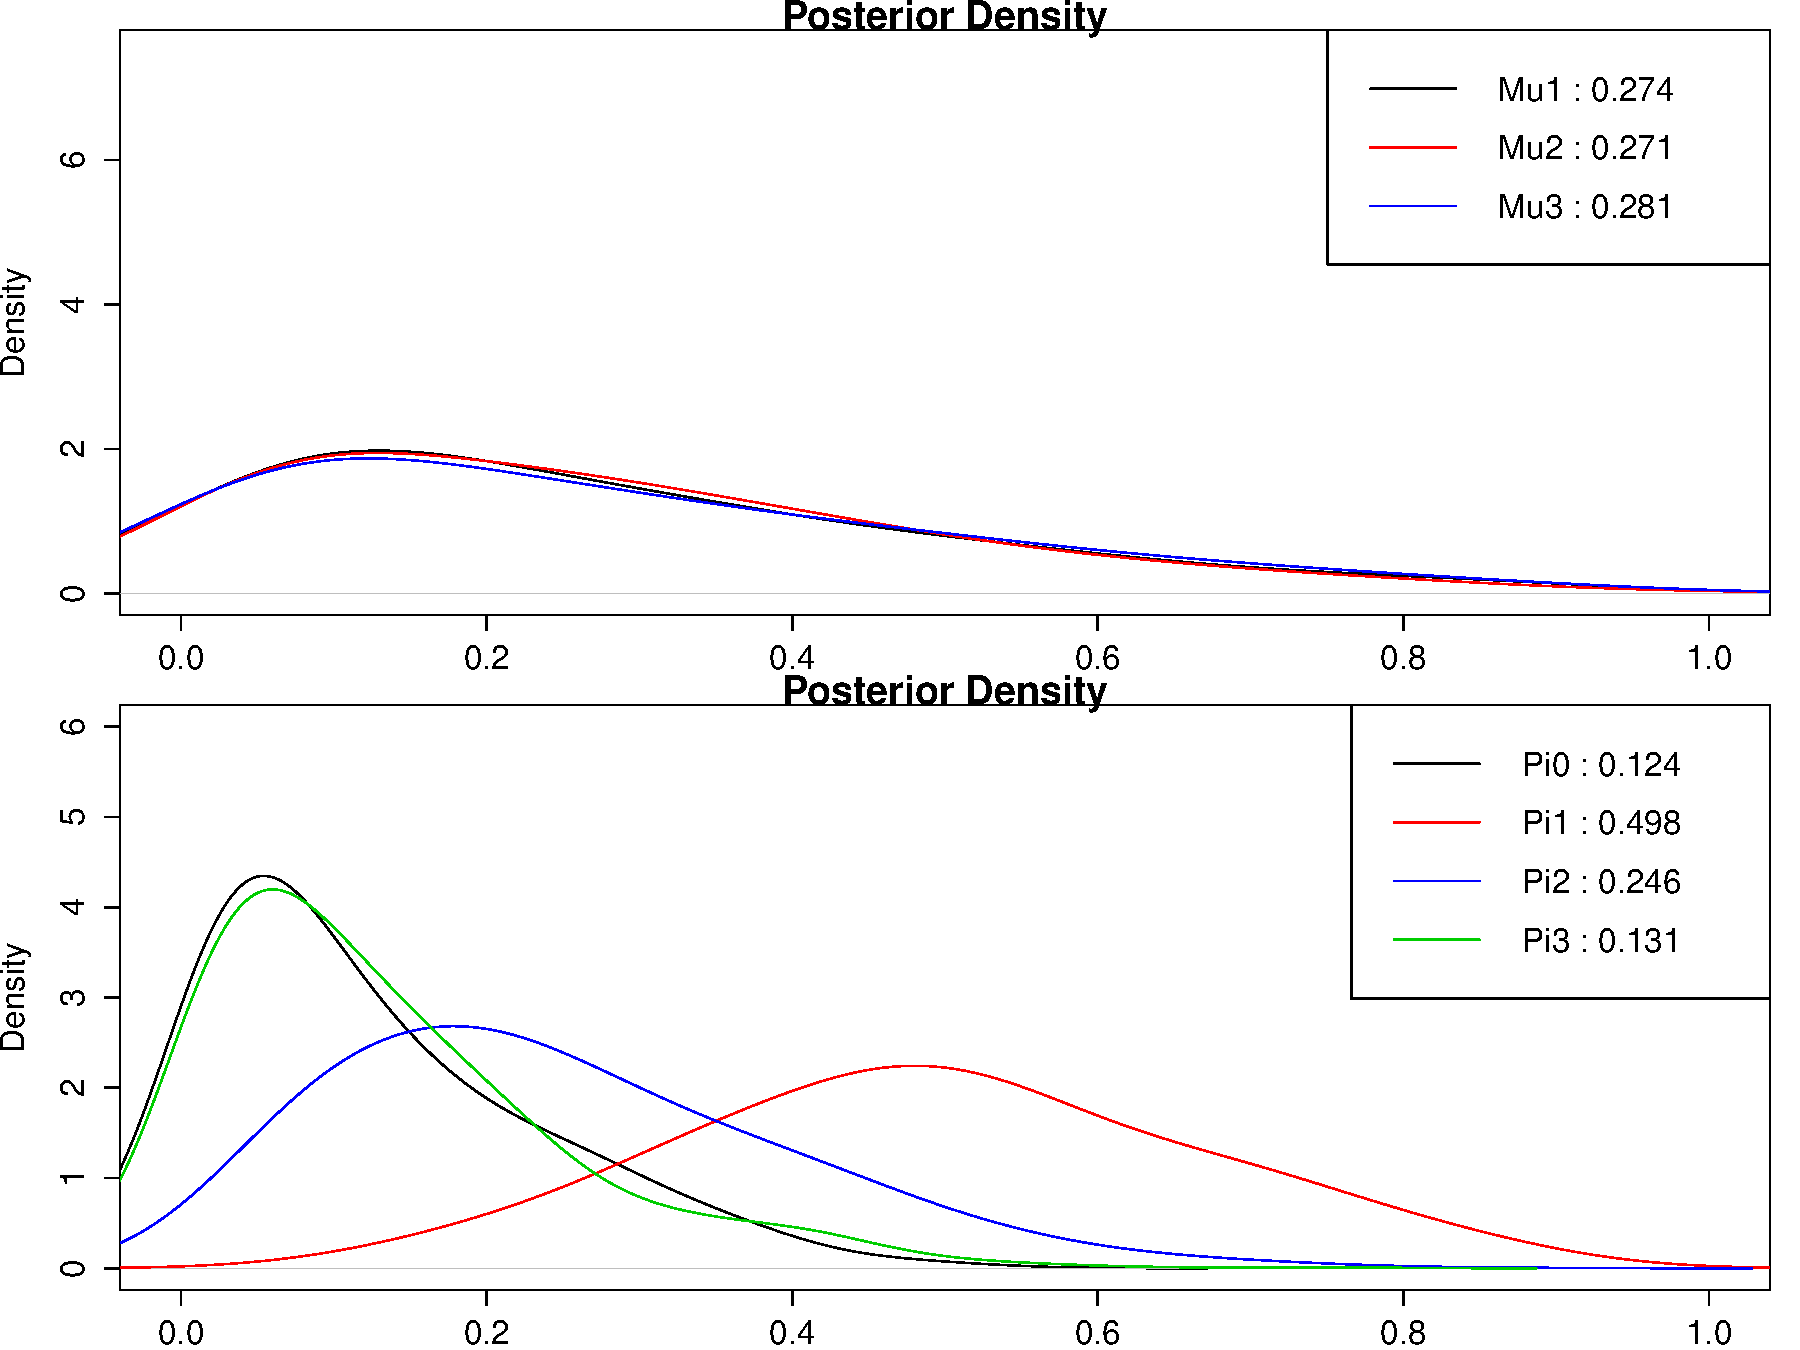
\includegraphics[scale=0.5]{dirich_uniform_prior.pdf}
\captionof{figure}{Prior marginal density plot }
\label{prior}
\end{center}


\subsection{The Likelihood $P(L|\mu, \pi)$}
\begin{align}
P(L | \mu, \pi) \nonumber \\ 
= & \int P(L, \phi | \mu, \pi) d \phi \nonumber \\ 
= & \int P(L | \phi, \mu, \pi) P(\phi | \mu,\pi) d \phi \nonumber \\ 
= & \int P(L | \phi) P(\phi | \mu,\pi) d \phi \nonumber \\ 
\approx & \frac{1}{H}\sum P(L | \phi_h) 
\end{align}
where $P(L | \phi_h)$ is the multinomial density of $L$ evaluated at $\phi_h$, which is sampled uniformly from the feasible region subject to constrains (5-7) with sample size $H$. \\

In fact, according to the prior specification, $(\pi_{Smax+1}, \ldots, \pi_K)=0$ then all corresponding $\phi_j$s are fixed at $0$ as well, thus only a small fraction of $\phi$ is actually sampled, that is, the dimension of $\phi$ shrinks from $J_1 = 2^K-1$ to $J_2={K \choose 1} + \ldots + {K \choose S_{max}}$.\\

\newpage

\subsubsection{Sampling Algorithm}
\begin{algorithm}[H]
\caption{Usample(n, $\mu, \pi_0, \pi_{0-}$)}
\begin{algorithmic}[1]
\If {neither $\mu, \pi_{0-}$ is NULL}
\State sample $\phi$ uniformly from feasible region defined by 
\begin{align*}
\phi > & 0\\
B \phi = & \pi_{0-}/\pi_0\\ 
C \phi = & \mu/\pi_0
\end{align*}
\ElsIf {only $\mu$ is NULL}
\State sample $\phi$ uniformly from feasible region defined by 
\begin{align*}
\phi > & 0\\
B \phi = & \pi_{0-}/\pi_0
\end{align*}
\Else
\State sample $\phi$ uniformly from feasible region defined by 
\begin{align*}
\phi > & 0\\
C \phi = & \mu/\pi_0
\end{align*}
\EndIf
\State {\bf return} $n$ samples of $\phi$
\end{algorithmic}
\end{algorithm}


\begin{algorithm}[H]
\caption{SampleByBlock($n_{Iter}, n_{Burn}, L, \mu_{init}, \pi_{init}, \sigma$)}
\begin{algorithmic}[1]
\State Initialize $\mu^{(0)} = \mu_{init}$, $\pi^{(0)} = \pi_{init}$
\For {$t \in 1 \text{ to } (n_{Iter} + n_{Burn})$}
\State $\phi = \text{Usample} (1, \mu=\text{NULL}, (\pi_0,\pi_{0-})=\pi^{(t-1)})$
\State $\mu^* = \pi_0^{(t-1)} C \phi $
\State $\alpha = \frac{P(L, \mu^*, \pi^{(t-1)} )}{P(L, \mu^{(t-1)}, \pi^{(t-1)} )}$
\State $\mu^{(t)} = \mu^*$ with probability $\max(1, \alpha)$; other wise, $\mu^{(t)} = \mu^{(t-1)}$
\State $\pi^*_{0} = \text{logit}^{-1}[logit(pi_{0}^{(t-1)}) + \epsilon]$, where $\epsilon \sim $ N$(0, \sigma)$.
\State $\phi = \text{Usample} (1, \mu=\mu^{(t)}, \pi_0=\pi^*_{0},\pi_{0-}=\text{NULL})$
\State $\pi^*_{0-} = \pi^*_{0} B \phi$
\State $\pi^* = (\pi^*_{0}, \pi^*_{0-})$
\State $\alpha = \frac{P(L, \mu^{(t)}, \pi^* )}{P(L, \mu^{(t)}, \pi^{(t-1)} )}$
\State $\pi^{(t)} = \pi^*$ with probability $\max(1, \alpha)$; other wise, $\pi^{(t)} = \pi^{(t-1)} $
\EndFor
\State {\bf return} $\mu^{(n_{Burn}+1)}$ to $\mu^{(n_{Burn} + n_{Iter})}$ and $\pi^{(n_{Burn}+1)}$ to $\pi^{(n_{Burn} + n_{Iter})}$
\end{algorithmic}
\end{algorithm}

\newpage
\section{Model with Measurement Error}
Let $M$ be the observed measurement, and $L$ be the latent true state, with $\gamma$ and $\delta$ representing the TPR and FPR.
\begin{align*}
P(\mu, \pi , \gamma, \delta|M) \propto & P(M, \mu, \pi, \gamma, \delta) \\
= & P(M | \mu, \pi, \gamma, \delta) P(\mu, \pi, \gamma, \delta) \\
= & \sum_{L \in \mathbb{L}}  P(M, L | \mu, \pi, \gamma, \delta) P(\mu, \pi, \gamma, \delta) \\ 
= & \sum_{L \in \mathbb{L}} \big[ P(M | L, \gamma, \delta) P(L | \mu, \pi) \big ] P(\mu, \pi) P(\gamma) P(\delta) \\ 
\end{align*}
where $\mathbb{L}$ is the set of all possible and allowed values of L, and
\begin{align*}
 P(M | L, \gamma, \delta) = & \prod_{k=1}^K P(M_k | L_k, \gamma, \delta) \text{\ \ (conditional independence assumption)}\\
 = & \prod_{k=1}^K (\gamma^{L_k} \delta^{1-L_k})^{M_k} [(1-\gamma)^{L_k} (1-\delta)^{1-L_k}]^{1-M_k}
\end{align*}
$P(\gamma)$ and $ P(\delta)$ are beta priors, and $P(L | \mu, \pi)  P(\mu, \pi)$ is defined in the same way as in previous section.


\subsection{Sampling Algorithm}

%\begin{table}[htbp]
%\begin{adjustwidth}{-0.5in}{-1in}
%\resizebox{0.7\textwidth}{!}{\begin{minipage}{\textwidth}
%\caption{Summary of the model coefficients and standard error estimates}
%\label{tab: coef}
%
%\begin{tabular}{llllll|lllll} 
%\hline 
% \\
%\hline \\
%\end{tabular}
%\end{minipage}}
%\end{adjustwidth}
%\end{table}





\newpage
\section*{Reference}
1. Smith RL . “Efficient Monte-Carlo Procedures for Generating Points Uniformly Dis- tributed over Bounded Regions.” Operations Research, 32(6), 1296–1308 (1984).\\ 
2. Van den Meersche, Karel, K. E. R. Soetaert, and D. J. Van Oevelen. "xsample (): an R function for sampling linear inverse problems." Journal of Statistical Software 30 (2009).


\end{document}






















